\clearpage
\section{How Graph Size and Degree Affect Distributional Generalization}
\label{sec:factorial}
\paragraph{Motivation and controlled design.}
The preceding robust study found an occupancy-event TV lower bound of .894
on one 512-node degree-100 regular graph, while supporting approximate
conditional equivalence in seven small graphs. To separate observed size and
degree effects, we preregistered a new factorial study with all fifteen
historical epoch-120 checkpoints, without further training. The primary grid
crosses $n\in\{128,256,512,1024\}$ and $d\in\{3,10,50,100\}$, with three
independent connected labeled regular realizations in each cell. Exact vertex
counts, all degrees, simplicity, connectivity, seeds and distinct labeled
edge hashes were audited. The generator is not assumed exactly uniform over
all regular graphs, and three realizations cannot characterize that population.

Cost pilots fixed 500 fresh testing attempts per generator and a separate
125-attempt explanatory holdout. The secondary cohort has one heterogeneous
graph per cell of $n\in\{128,1024\}$ crossed with all four degrees, including
low-degree vertices, intermediate degrees and a small hub group. Degree and
palette histograms are archived. A third stratum replicates the exact
historical edge list using new independent seeds. Every local palette remains
$\{0,\ldots,d(v)\}$; no global-degree input or new action shield is introduced.

\paragraph{Complete-law tests and estimands.}
An observation is a complete labeled coloring vector, not a vertex. The
principal law conditions on proper completion by round 128; improper
completion, cutoff and technical error remain separate outcomes. We reuse
the frozen omnibus V2, its honest selection/evaluation split, local and
pair/triple witnesses, structural features and characteristic full-vector
kernel unchanged. Joint label permutations number 19,999, with inclusive
ties and plus-one p-values. Holm controls the 720 primary graph--checkpoint
hypotheses at .05. The 120 irregular and 15 historical-replication hypotheses
have separate families. The old Hamming MMD is evaluated on exactly the same
new bank in its own method family. Event, completion and independent witness
analyses also have separate families; no .05 FWER is asserted over their union.

The primary structural events are
\[
 A_{n,d}=\{U(X)\le d\},\qquad
 T_{n,d}=\{\text{color }d\text{ occurs}\}.
\]
The first means that at least one palette color is absent, which need not be
the top color. A saturated stratified binomial model has one event probability
per fixed graph/generator bank, conditional on its valid count. Architecture
summaries average the three graphs and five fixed checkpoints equally, counting
the shared teacher bank once. We preregistered 1,800 cell, adjacent-size,
adjacent-degree and probability-scale interaction contrasts. Elementary exact
binomial intervals and weighted independent-run Hoeffding intervals receive
.025 error budgets each; their intersections cover all contrasts simultaneously
with probability at least .95. These are fixed-cohort intervals, rather than
population intervals assuming many independent graphs or trained networks.

An event-difference interval $[l,u]$ yields a same-graph lower bound
$\operatorname{TV}(P_L,P_M)\ge\max(0,l,-u)$. Lower bounds do not order the
unknown true TV distances. Across sizes the vector spaces also differ, so
we compare consistently defined functions and events, rather than computing
cross-dimensional TV. Small MMD or a nonrejection supplies no useful TV upper
bound without an additional quantitative argument.

\paragraph{Results across size and degree.}
Table~\ref{tab:factorial-tests} retains all gains and losses of V2 on the
same new samples. Counts are not distance estimates and cannot be directly
ranked against the earlier 265-comparison architecture cohorts.
\begin{table}[t]
\centering\small
\begin{tabular}{lrrrr}
\toprule Architecture & V2 & Old MMD & V2 only & MMD only\\
\midrule
E1 NORMALIZED & 115/240 & 49/240 & 66 & 0 \\
DeepSets & 170/240 & 121/240 & 49 & 0 \\
LocalPaletteTransformer & 180/240 & 174/240 & 6 & 0 \\
\bottomrule
\end{tabular}
\caption{Regular factorial cohort: 240 comparisons per architecture;
Holm is applied across all 720 hypotheses separately for each method.}
\label{tab:factorial-tests}
\end{table}

Figures~\ref{fig:factorial-discrepancy}--\ref{fig:factorial-degree}
give the full event-effect matrix and its slices with simultaneous intervals.
These are measured changes in occupancy probability, not merely changes in
test power. Top-color appearance is separately reported in
Figure~\ref{fig:factorial-top}, including regimes where $U\le d$ is nearly
certain under both generators. We impose no monotone full-law TV interpretation.

For E1 at degree 50, the top-appearance risk difference is
-0.239 [-0.307, -0.170] at 128 vertices and
-0.004 [-0.031, +0.023] at 1,024 vertices.
Thus this observable discrepancy attenuates in that regime. At degree 100,
the adjacent 256-to-512 change in the missing-color risk difference is
+0.481 [+0.384, +0.579].
Already at $n=128,d=100$, the top-appearance difference is
-0.610 [-0.679, -0.541], despite a missing-color
risk difference of +0.000 [-0.024, +0.024].
The two observables therefore supply different information; an uninformative
missing-color event is not evidence of equal complete laws.
The simultaneous cell bands imply a reduction of at least 0.138
in the absolute top-appearance risk difference between 128 and 1,024 vertices
at degree 50. This conservative deduction orders that fixed-cohort observable,
not the unknown complete-law TV distances.

\begin{table}[t]
\centering\small
\begin{tabular}{lrr}
\toprule Architecture & Four-corner interaction for $A$ & Simultaneous interval\\
\midrule
E1 NORMALIZED & +0.603 & [+0.479, +0.699] \\
DeepSets & +0.001 & [-0.094, +0.097] \\
LocalPaletteTransformer & +0.201 & [+0.093, +0.299] \\
\bottomrule
\end{tabular}
\caption{Extreme-level difference-in-differences of event risk differences.
All adjacent interactions and individual-checkpoint contrasts are archived.
This is a probability-scale fixed-cohort interaction, not causal identification.}
\label{tab:factorial-interaction}
\end{table}

\paragraph{Independent replication and checkpoint variation.}
Archived historical data exactly reproduce .008 versus 1.000 for $U\le100$
in \texttt{normalized-s41000} on the original graph. They are never pooled
with new outcomes. Across the three new $n=512,d=100$ graphs and five E1
checkpoints, the smallest simultaneous event-TV lower bound is 0.023.
Using both preregistered events, every one of these fifteen pairs has TV at
least 0.078; maximizing two bounds from their same simultaneous family
preserves its coverage. The effect is heterogeneous across checkpoints.
Figures~\ref{fig:factorial-used}--\ref{fig:factorial-replication}
retain occupancy distributions, all five training replicas and the independent
replication on the original edge list. Leave-one-graph/checkpoint ranges are
sensitivity analyses rather than population confidence intervals.

Architecture-level missing-color differences at $n=512,d=100$ are E1 NORMALIZED: +0.639 [+0.570, +0.703]; DeepSets: +0.038 [-0.031, +0.107]; LocalPaletteTransformer: +0.294 [+0.225, +0.363]. These contrasts retain a common probability scale and are not rankings by rejection frequency.

\paragraph{Mechanistic evidence.}
Read-only observers record proposals, participation, exact availability
references, accepted colors and terminal classes on eight fresh trajectories
per generator and selected graph. Every checkpoint is also probed on identical
teacher states with midpoint grids of 1,024 and 4,096 private uniforms. A grid
zero is not a proof of zero operational mass. Candidate biases and independent
terminal event estimates are related in Figure~\ref{fig:factorial-candidates};
the proposal/COMMIT accounting remains descriptive, not an intervention or
causal mediation estimate.

At an all-uncolored nonisolated vertex, MAX returns the same finite message
type regardless of neighbor multiplicity. Thus at fixed $K$, the initial
candidate function is independent of $n$ and the particular regular edge
realization. This does not imply invariance of subsequent states or terminal
laws. With independent initial candidates of law $q$, independent participation
of probability $p$ and the exact conflict COMMIT rule, the unconditional first-round reference is
\[
 \Pr(v\text{ confirms }c)=p q_c(1-p q_c)^d.
\]
Every neighbor must avoid participating with candidate $c$. This nonlinear
relation does not make different vertices' confirmations independent, and
we do not assume the learned COMMIT head always equals that exact rule.
The ideal teacher has $p=1/2$, $q_c=1/(d+1)$.
Ideal continuous teacher randomness also has global color-permutation
symmetry on regular graphs, implying a uniform single-vertex marginal and
$E_L[U]=K P_L(T)$ conditional on the invariant completion event. It does not
imply uniformity over proper colorings on arbitrary regular graphs. The ideal
argument is distinct from a bitwise floating-point certificate.

The earlier clique result instead uses transitivity of vertex permutations
on the proper bijective colorings. Conditional uniformity there can coexist
with nonuniform candidate proposals. General regular graphs admit multiple
color-class profiles and lack that transitivity, so clique equality does
not establish general complete-law transfer beyond those symmetry conditions.

\paragraph{Exploration and limitations.}
Six binomial predictor forms---size, degree/palette, $n/K$, density, additive
and interaction---are compared with checkpoint intercepts and whole-graph
replicate holdouts. Their predictive ranking is not claimed as confirmatory
causal variable selection. Structural projections, per-color profiles and
MMD effects retain their stated scale and uncertainty limitations. Selected
events are validated on the independent explanation bank; prospectively
measuring every color permits simultaneous rather than naive selected-color
intervals. A small normalized occupancy-mean difference can coexist with a
large discrepancy of an occupancy-tail event.

The distinction between initial proposals and terminal laws is quantitative:
for E1 checkpoint 41004, the initial 4,096-point top-color mass
at $K=101$ is 0.000000, yet the mean final top-color appearance across
the three new priority graphs is 0.813.
Availability changes along a trajectory; a zero initial grid mass cannot
certify absence in every later state.

For an illustrative E1 NORMALIZED checkpoint
\texttt{normalized-s41000} on $n=1024,d=100$,
the held-out event \texttt{used\_colors}$\le 100$ has probabilities
0.000 versus 1.000, risk difference
+1.000 with simultaneous interval
[+0.830,+1.000], giving TV at least 0.830.

For an illustrative DeepSets checkpoint
\texttt{deepsets-s41004} on $n=1024,d=100$,
the held-out event \texttt{mean\_color}$\le 48.975586$ has probabilities
0.032 versus 0.968, risk difference
+0.936 with simultaneous interval
[+0.697,+0.998], giving TV at least 0.697.

For an illustrative LocalPaletteTransformer checkpoint
\texttt{transformer-s41000} on $n=1024,d=10$,
the held-out event \texttt{class\_entropy}$\le 2.3934074$ has probabilities
0.000 versus 1.000, risk difference
+1.000 with simultaneous interval
[+0.830,+1.000], giving TV at least 0.830.

Here mean color uses the numeric labels and class entropy uses natural logs.
Each witness was selected only on the main bank and measured on the independent
125-run holdout. Simultaneous exact-binomial bounds over the entire 855-witness
family allow choosing these examples after measurement. They illustrate
different observable discrepancies; they are not universal explanatory or
causal rankings of features.

For heterogeneous prefix lists, every completed assignment obeys
$U\le\min_t[t+\#\{v:d(v)\ge t\}]$. Five of the eight secondary graphs
therefore force $U\le d$ under every generator (for example $U\le44$ on the
1,024-node degree-100 graph). Agreement on that event has no discriminating
content in these cells; the full test, top-color event and other profiles
remain informative targets. Irregular results are not pooled with regulars.

In the separate 120-hypothesis irregular family, the V2/old-MMD rejection counts are E1 NORMALIZED: 7/40 versus 0/40; DeepSets: 26/40 versus 21/40; LocalPaletteTransformer: 37/40 versus 33/40. Figure~\ref{fig:factorial-irregular} reports top-color appearance differences,
which retain information when missing-color occupancy is forced by the lists.
Its fixed-checkpoint mean intervals are linear images of the original
simultaneous elementary CP bounds; the shared teacher enters once. One graph
per irregular cell limits generalization, and maximum degree does not specify
its full palette-capacity profile.

\paragraph{Exploratory explanations with simultaneous threshold selection.}
The original single-event explanation selector can overfit categorical
patterns even when an independently evaluated global statistic rejects.
For E1 checkpoint 41003 on the 1,024-node degree-50 graph r0, it fitted 500
distinct triples. Its event covered 250/250 teacher versus 0/250 model rows
during selection, 1/250 versus 0/250 evaluation rows, and 0/125 versus 1/125
reserved rows. The honest holdout correctly refused to validate that event.
We preserve this failure and all original omnibus results.

After inspecting it, we added an explicitly exploratory analysis using all 625
original attempts and only the seven scalar functions frozen before sampling.
For each of 57 graphs, 16 generators and 7 functions, the DKW radius is
$\epsilon_N=\sqrt{\log(2\cdot6384/.05)/(2N)}$, clipped at 1. A union bound
covers all 6,384 CDFs and all thresholds simultaneously with probability at
least .95, with the shared teacher counted once. Subtracting clipped bands
allows data-dependent choice of a predefined function and threshold without
a naive selected-event interval. This is a new separate confidence family,
not independent confirmation or a revision of the primary rejection counts.

Positive full-law TV lower bounds in the main cohort are E1 NORMALIZED: 119/240 overall, including 109/115 global rejections; DeepSets: 167/240 overall, including 167/170 global rejections; LocalPaletteTransformer: 180/240 overall, including 180/180 global rejections.
All fifteen E1 comparisons at $n=1024,d=50$ have positive bounds in this
family, despite nearly uninformative missing-color and top-appearance events.
Figure~\ref{fig:factorial-cdf} and Table~\ref{tab:factorial-cdf} give
examples from the same graph r0. Normalized class entropy detects a strong
checkpoint-specific shift, while numeric mean color also distinguishes two
checkpoints for which the original categorical explanation failed.
The individual CDF radius is .09980 at 625 valid runs; the report archives
probability and difference bands for all seven metrics and all 855 comparisons,
including zero bounds. Noninjective projections cannot establish equality
or upper bounds on full-law TV.
\begin{table}[t]
\centering\small
\begin{tabular}{llrrrr}
\toprule E1 seed & Metric $\phi$ & Threshold $t$ & $P_L$ & $P_M$ & TV lower\\
\midrule
41000 & $H/\log K$ & 0.99604342 & 0.0320 & 0.9632 & 0.732 \\
41003 & $\bar c/d$ & 0.49783203 & 0.3680 & 0.6304 & 0.063 \\
41004 & $\bar c/d$ & 0.49800781 & 0.3792 & 0.6544 & 0.076 \\
\bottomrule
\end{tabular}
\caption{Exploratory events $\phi(X)\le t$ on the same $n=1024,d=50$
graph r0. Probabilities use 625 valid runs per generator; TV lower bounds
have simultaneous coverage at least .95 over the separate 6,384-CDF family.
$H$ is class entropy, $K=51$, and $\bar c$ is mean numeric color.}
\label{tab:factorial-cdf}
\end{table}

\paragraph{Separate exploratory candidate intervention.}
A prospectively recorded extra experiment replaces only the candidate
channel by exact local teacher proposals on the intervened policy's own
state. Learned participation, original COMMIT, checkpoints and cutoff are
unchanged; no safety mask is added. Across 60 of 60 planned cells
(all checkpoints on three new priority graphs and the historical graph),
the status is \texttt{complete}.
The sample count of 1,000 independent pairs per cell was selected exclusively
from a separate timing pilot, within the same total GPU budget. These observations do not enter the
original 720 hypotheses.

Common-random-number coupling, with independent pairs, gives simultaneous
upper bounds on conditional TV between the intervened policy $I$ and Luby;
paired outputs are never treated as independent two-sample observations.
The bound is at most .05 in 0/60 cells; approximate
restoration to the teacher law is therefore not established.
Original and intervention event intervals jointly support a positive
lower bound on $\operatorname{TV}(P_M,P_I)$ in
40/60 cells, with coverage at least .95.
We recorded 0 unsafe COMMIT decisions and did not repair them.
A large coupling upper bound does not prove residual discrepancy, since
the coupling need not be optimal. This controlled computational intervention
addresses the candidate channel; it does not identify complete mediation
or separate degree from palette causality.

A separate supplementary addendum was recorded after original witness
examples were inspected but before any intervention sample. It retains the
single honestly selected original event for each of all sixty cells and
uses its original independent holdout. Simultaneous CP bounds on 360 event,
mismatch and success probabilities, followed by direct fixed-event comparison
under the intervened policy and the triangle inequality,
give positive lower bounds on $\operatorname{TV}(P_M,P_I)$ in
43/60 cells. The simultaneous
coverage is at least .95 for this supplementary family; it is separate from
the preceding event-effect family, and no joint .95 guarantee is claimed
over their union. No new simulations or event reselection are involved.

The final ledger charged 10.185 of 12 GPU-process hours,
including pilots and diagnostic trajectories. Statistical analyses use CPU.
The audit checked 650,656 distinct new algorithm seeds,
without historical overlap, unchanged checkpoint/source hashes, a complete
teacher-bank replay, two omnibus replays and multiplicity recalculation.
Confirmation statuses are [570000, 0, 0, 0] in the order proper,
improper, cutoff and technical error. The protocol was committed as
\texttt{5633b547682b} before confirmation.

\paragraph{What We Can Prove, What We Observe, and What Remains Open.}
We can prove ideal teacher color symmetry, initial MAX-state invariance,
conditional permutation validity and stated coverage under independent runs.
We observe finite-cohort effects, interactions, replications and diagnostic
proposal/acceptance chains. Any candidate intervention has the separate
scope stated above. We cannot order all complete-law TV distances, generalize
three graphs and five trainings universally, or infer complete mediation
from association. On regular graphs, degree and palette size vary
together, leaving their separate causal effects unidentified. Previous
small-graph equivalence statements retain their original scope; large-graph
nonrejections establish no approximate equivalence.

\begin{figure}[p]
\centering
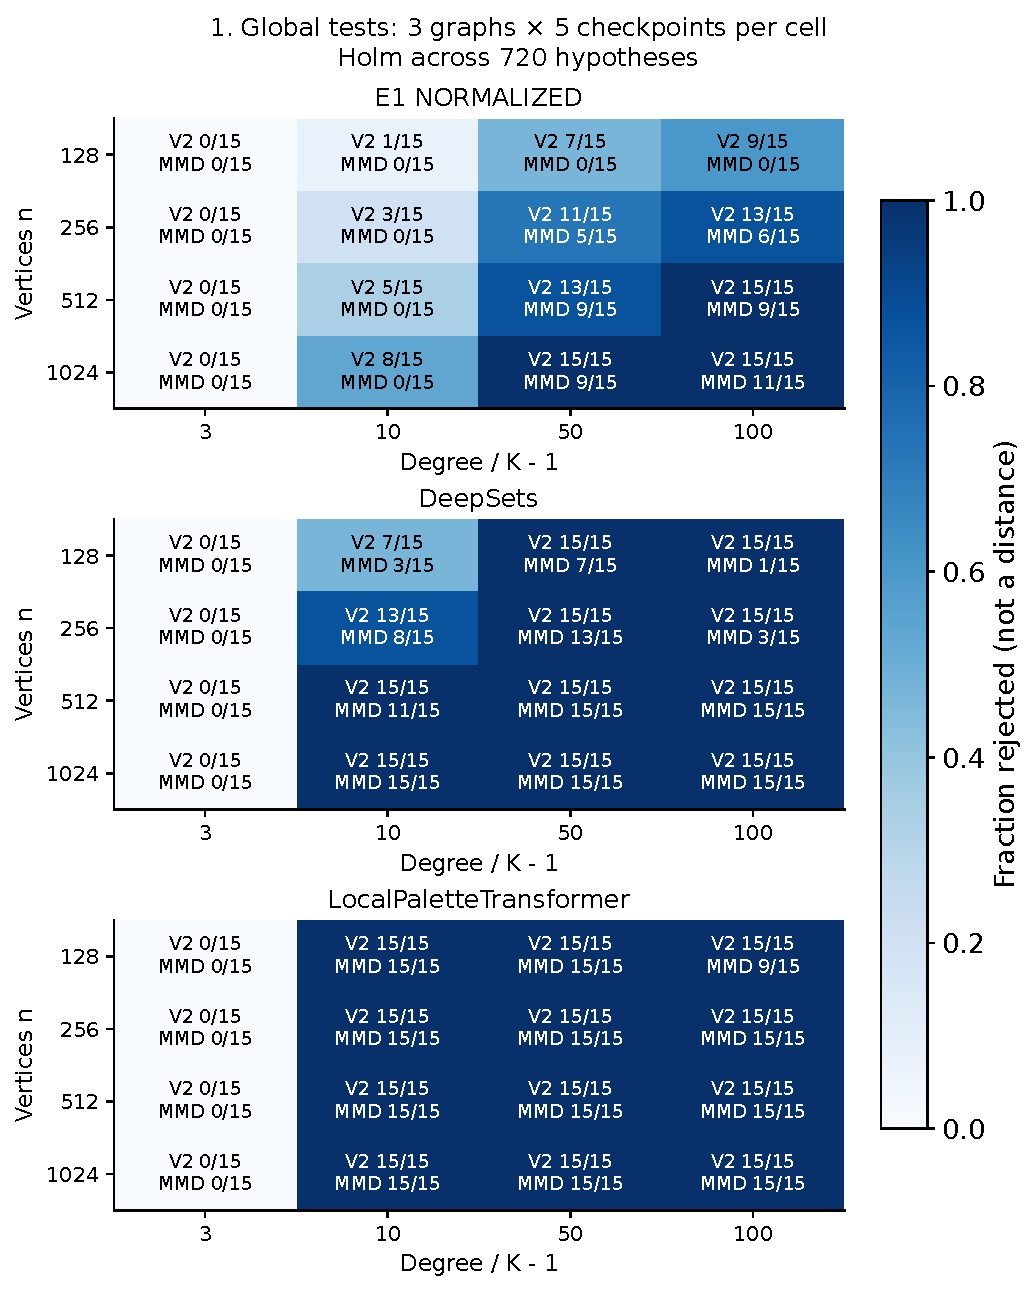
\includegraphics[width=\linewidth,height=.8\textheight,keepaspectratio]{figures/factorial-01-significance.pdf}
\caption{Global tests; each cell contains three graphs and five checkpoints. Rejection fractions are not distances.}
\label{fig:factorial-significance}
\end{figure}

\begin{figure}[p]
\centering
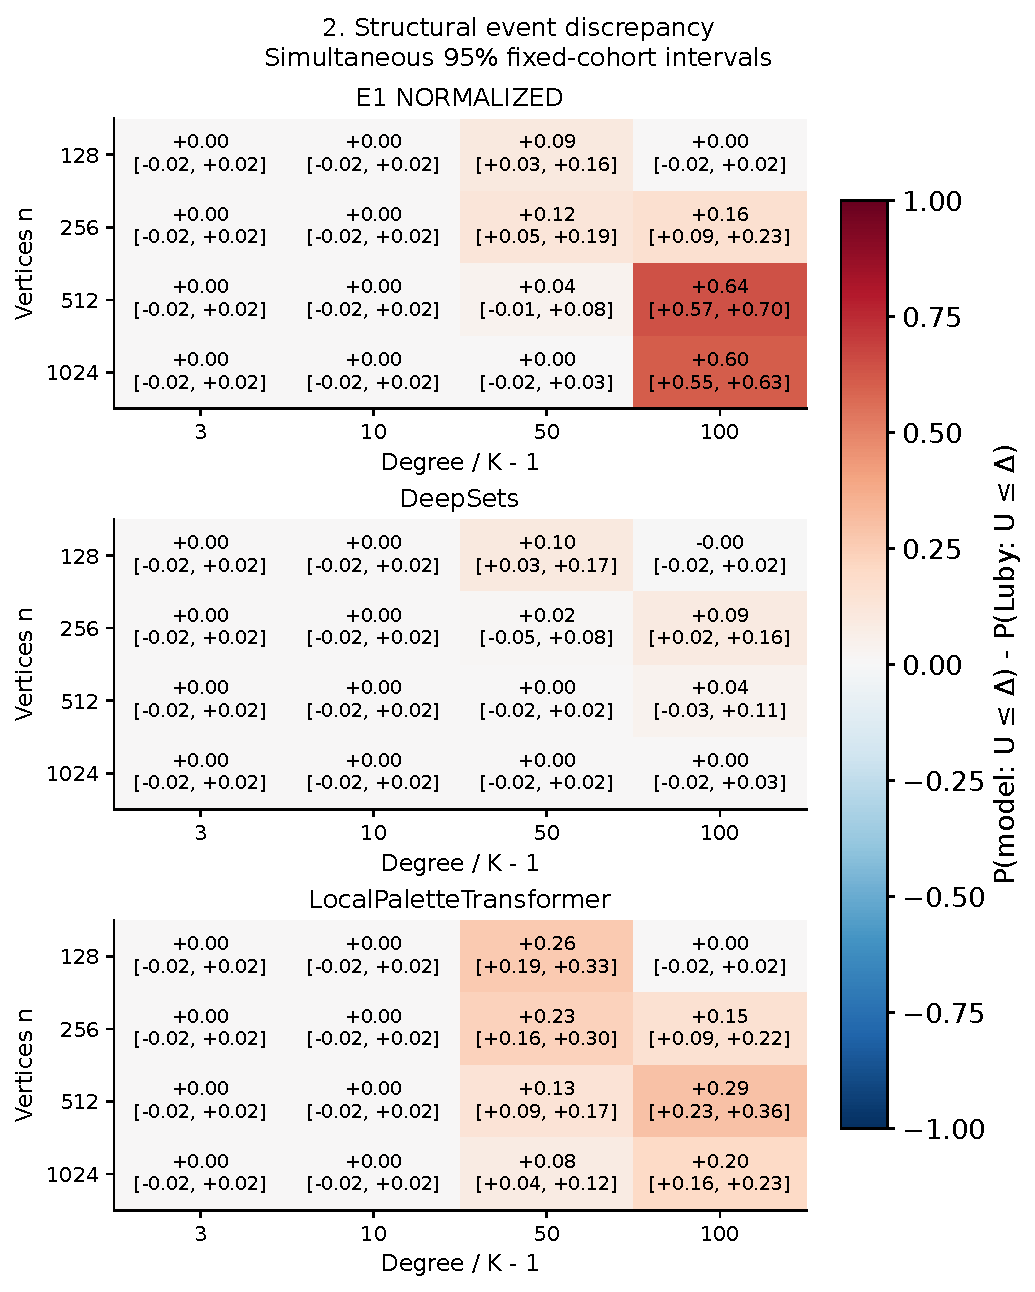
\includegraphics[width=\linewidth,height=.8\textheight,keepaspectratio]{figures/factorial-02-event-discrepancy.pdf}
\caption{Differences in the probability of using at most the degree many colors, with simultaneous fixed-cohort intervals.}
\label{fig:factorial-discrepancy}
\end{figure}

\begin{figure}[p]
\centering
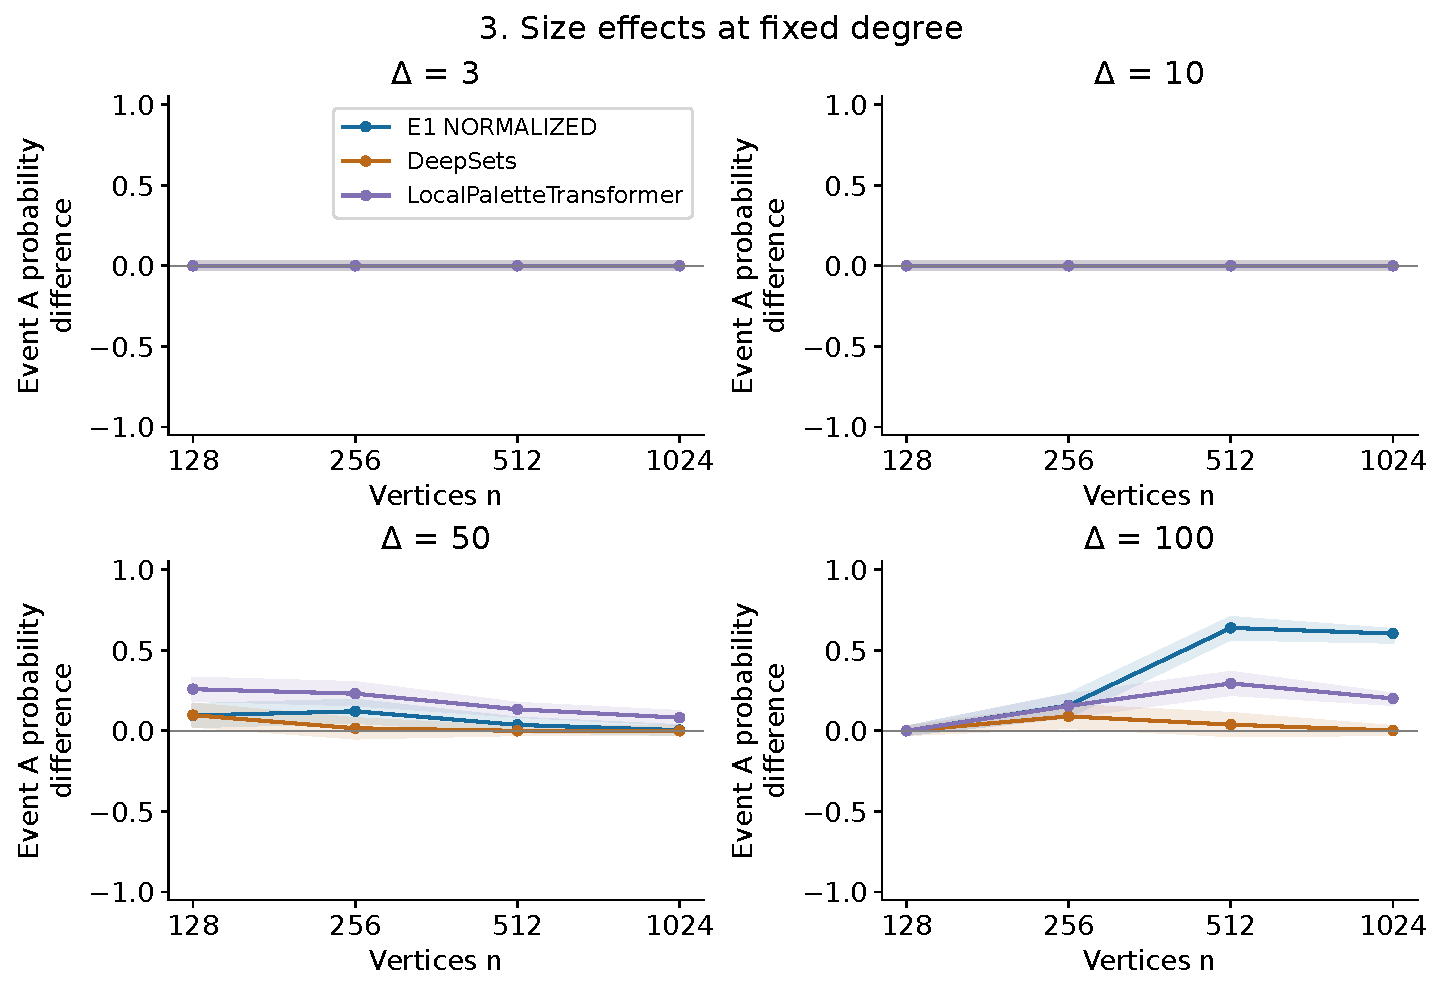
\includegraphics[width=\linewidth,height=.8\textheight,keepaspectratio]{figures/factorial-03-size-effect.pdf}
\caption{Size slices at fixed degree, with simultaneous fixed-cohort uncertainty.}
\label{fig:factorial-size}
\end{figure}

\begin{figure}[p]
\centering
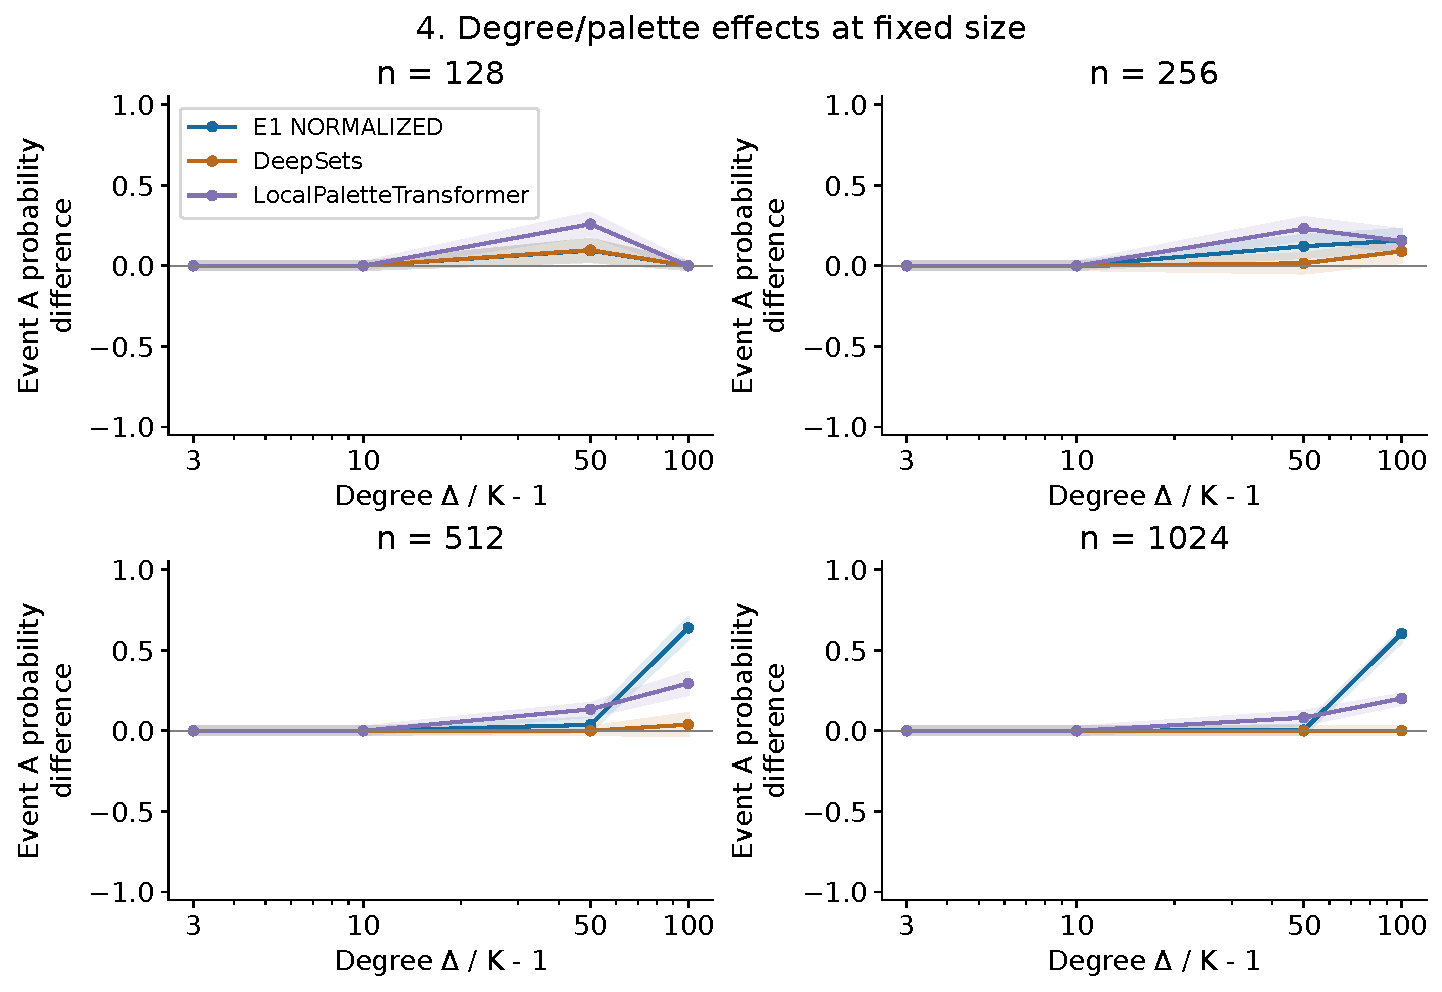
\includegraphics[width=\linewidth,height=.8\textheight,keepaspectratio]{figures/factorial-04-degree-effect.pdf}
\caption{Degree/palette slices at fixed size, without a monotone TV assumption.}
\label{fig:factorial-degree}
\end{figure}

\begin{figure}[p]
\centering
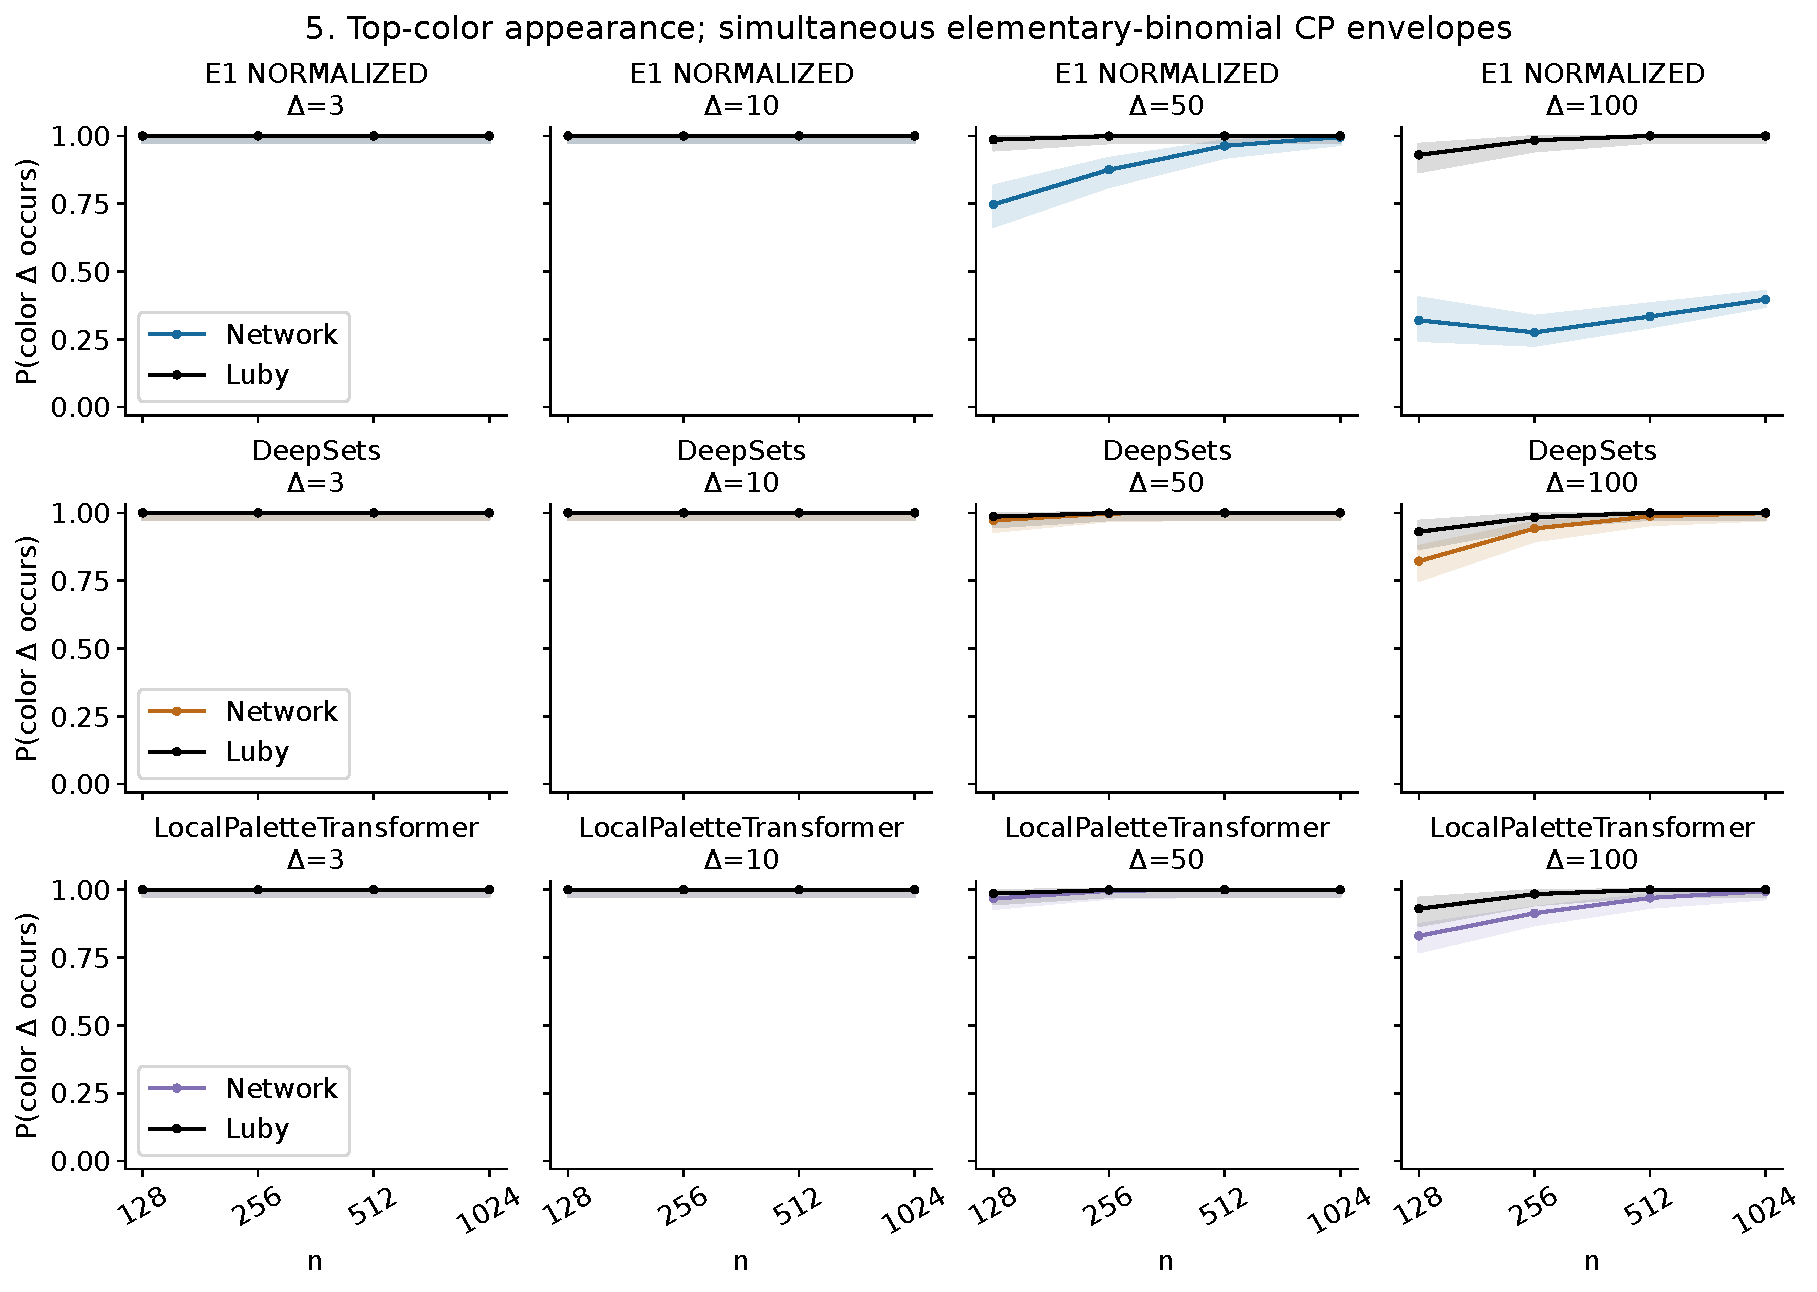
\includegraphics[width=\linewidth,height=.8\textheight,keepaspectratio]{figures/factorial-05-top-color.pdf}
\caption{Top-color appearance probabilities with simultaneous elementary CP envelopes.}
\label{fig:factorial-top}
\end{figure}

\begin{figure}[p]
\centering
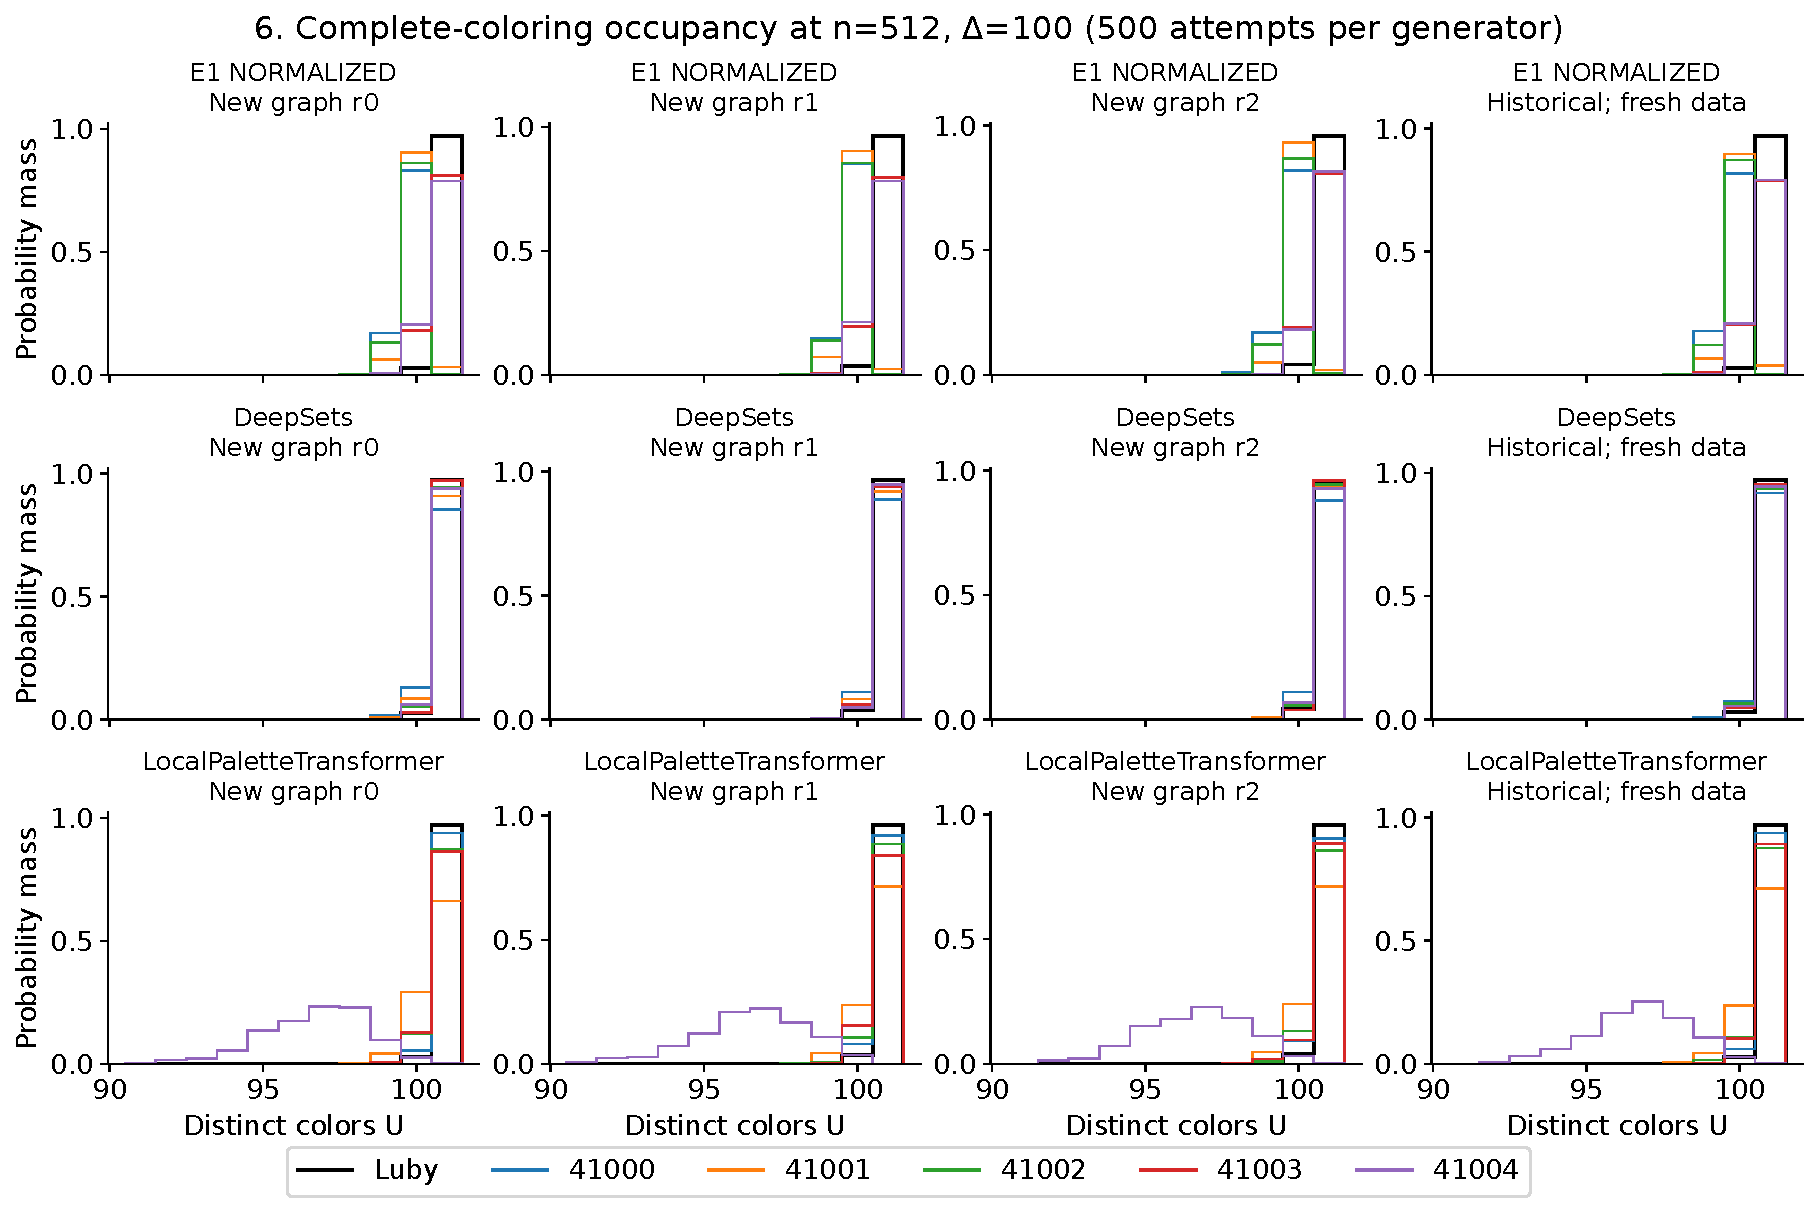
\includegraphics[width=\linewidth,height=.8\textheight,keepaspectratio]{figures/factorial-06-used-colors.pdf}
\caption{Occupancy distributions on three new priority graphs and the historical graph with independent fresh data.}
\label{fig:factorial-used}
\end{figure}

\begin{figure}[p]
\centering
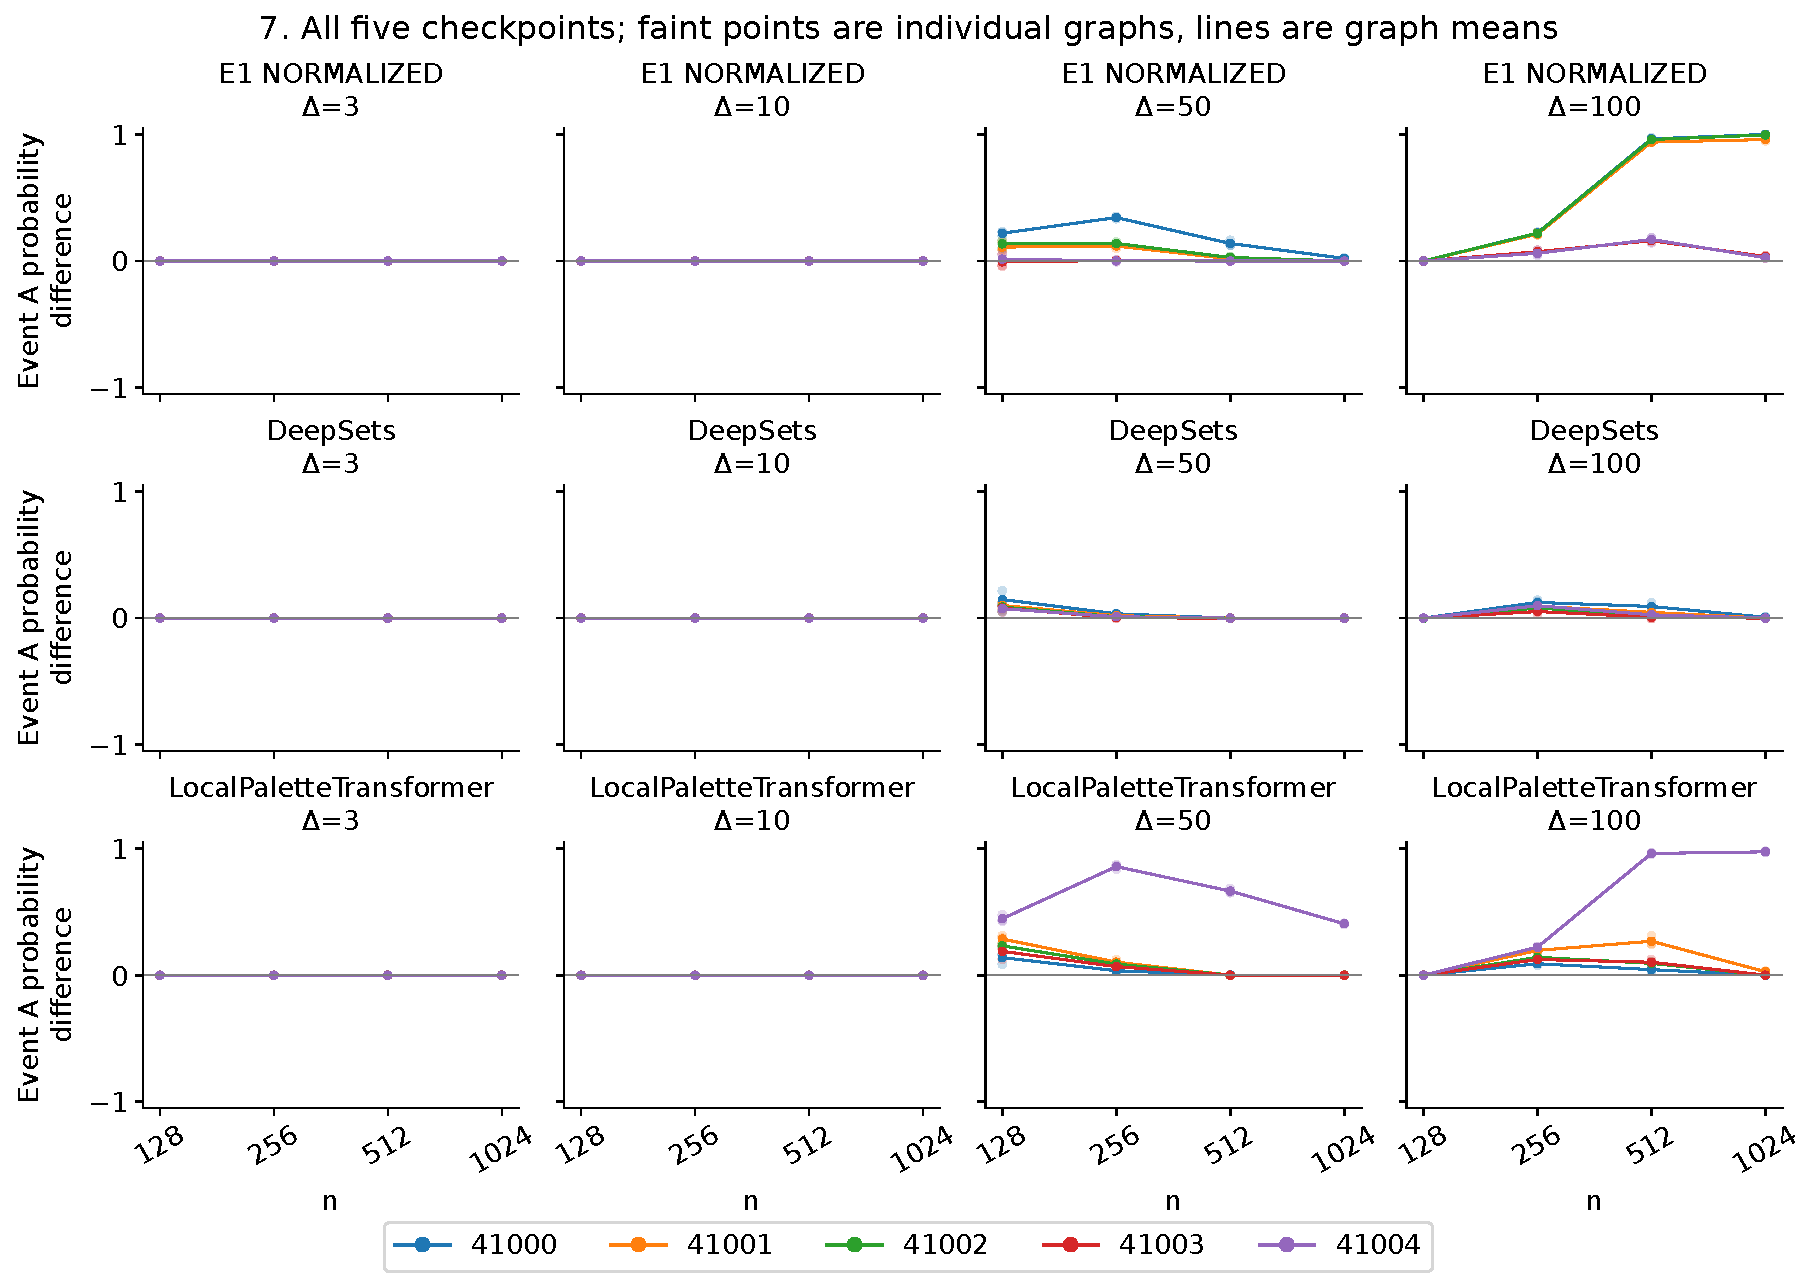
\includegraphics[width=\linewidth,height=.8\textheight,keepaspectratio]{figures/factorial-07-checkpoints.pdf}
\caption{All five checkpoints; faint points retain individual graph variation.}
\label{fig:factorial-checkpoints}
\end{figure}

\begin{figure}[p]
\centering
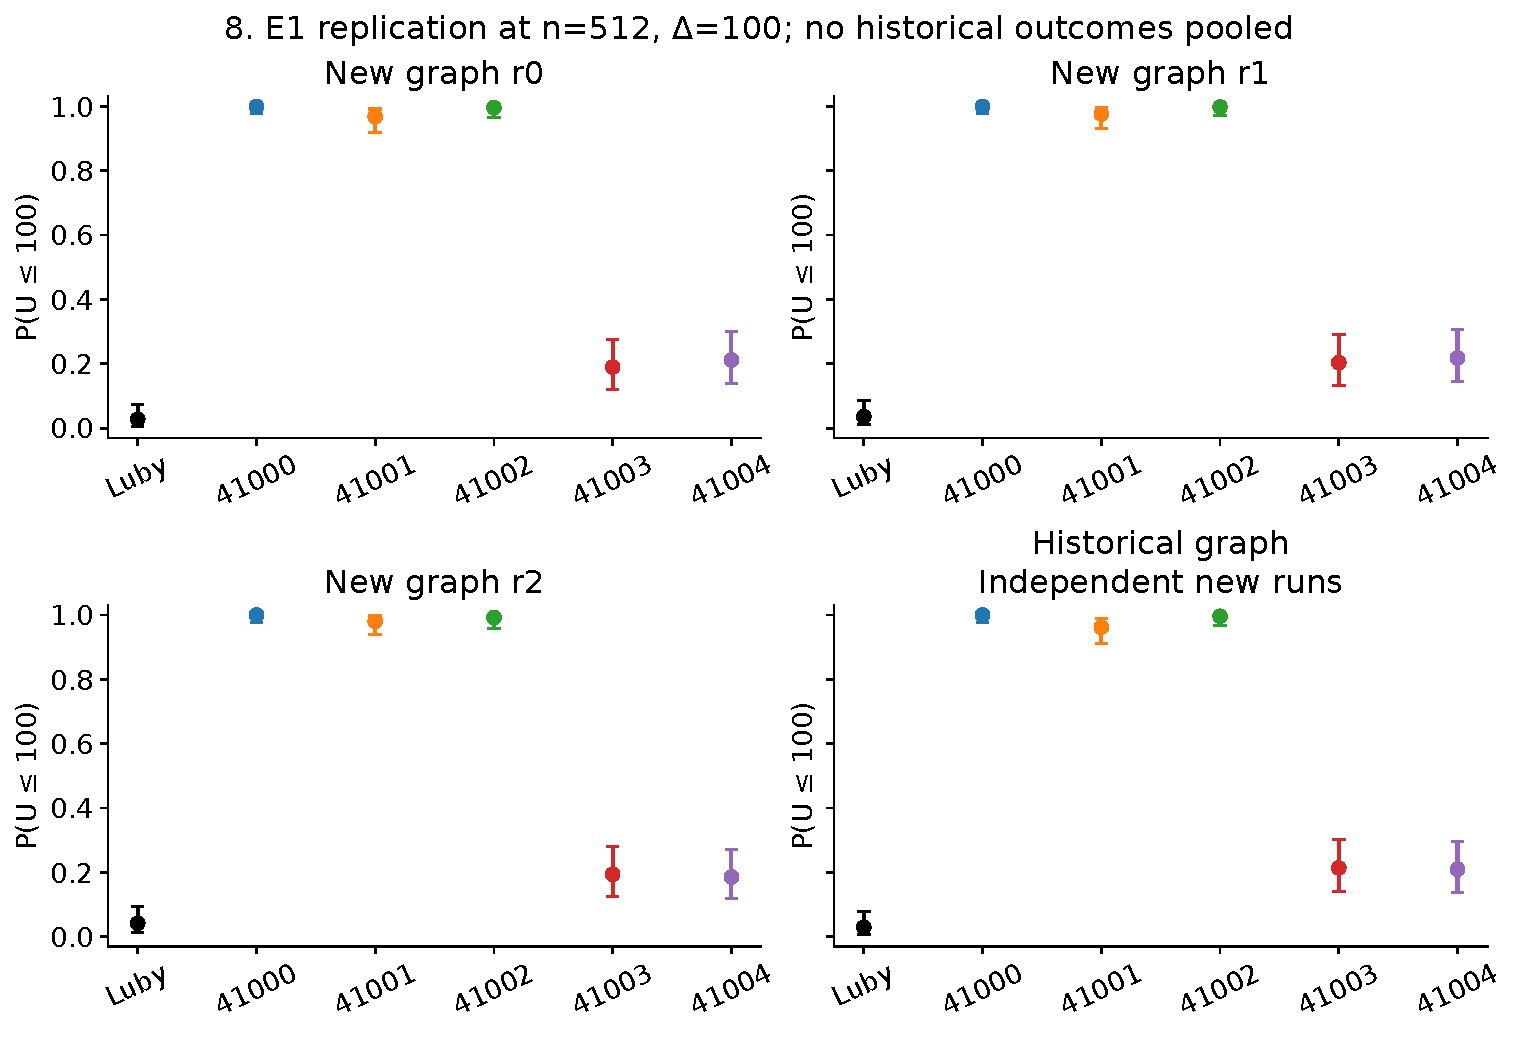
\includegraphics[width=\linewidth,height=.8\textheight,keepaspectratio]{figures/factorial-08-target-replication.pdf}
\caption{Independent priority-case E1 replications, without pooling historical outcomes.}
\label{fig:factorial-replication}
\end{figure}

\begin{figure}[p]
\centering
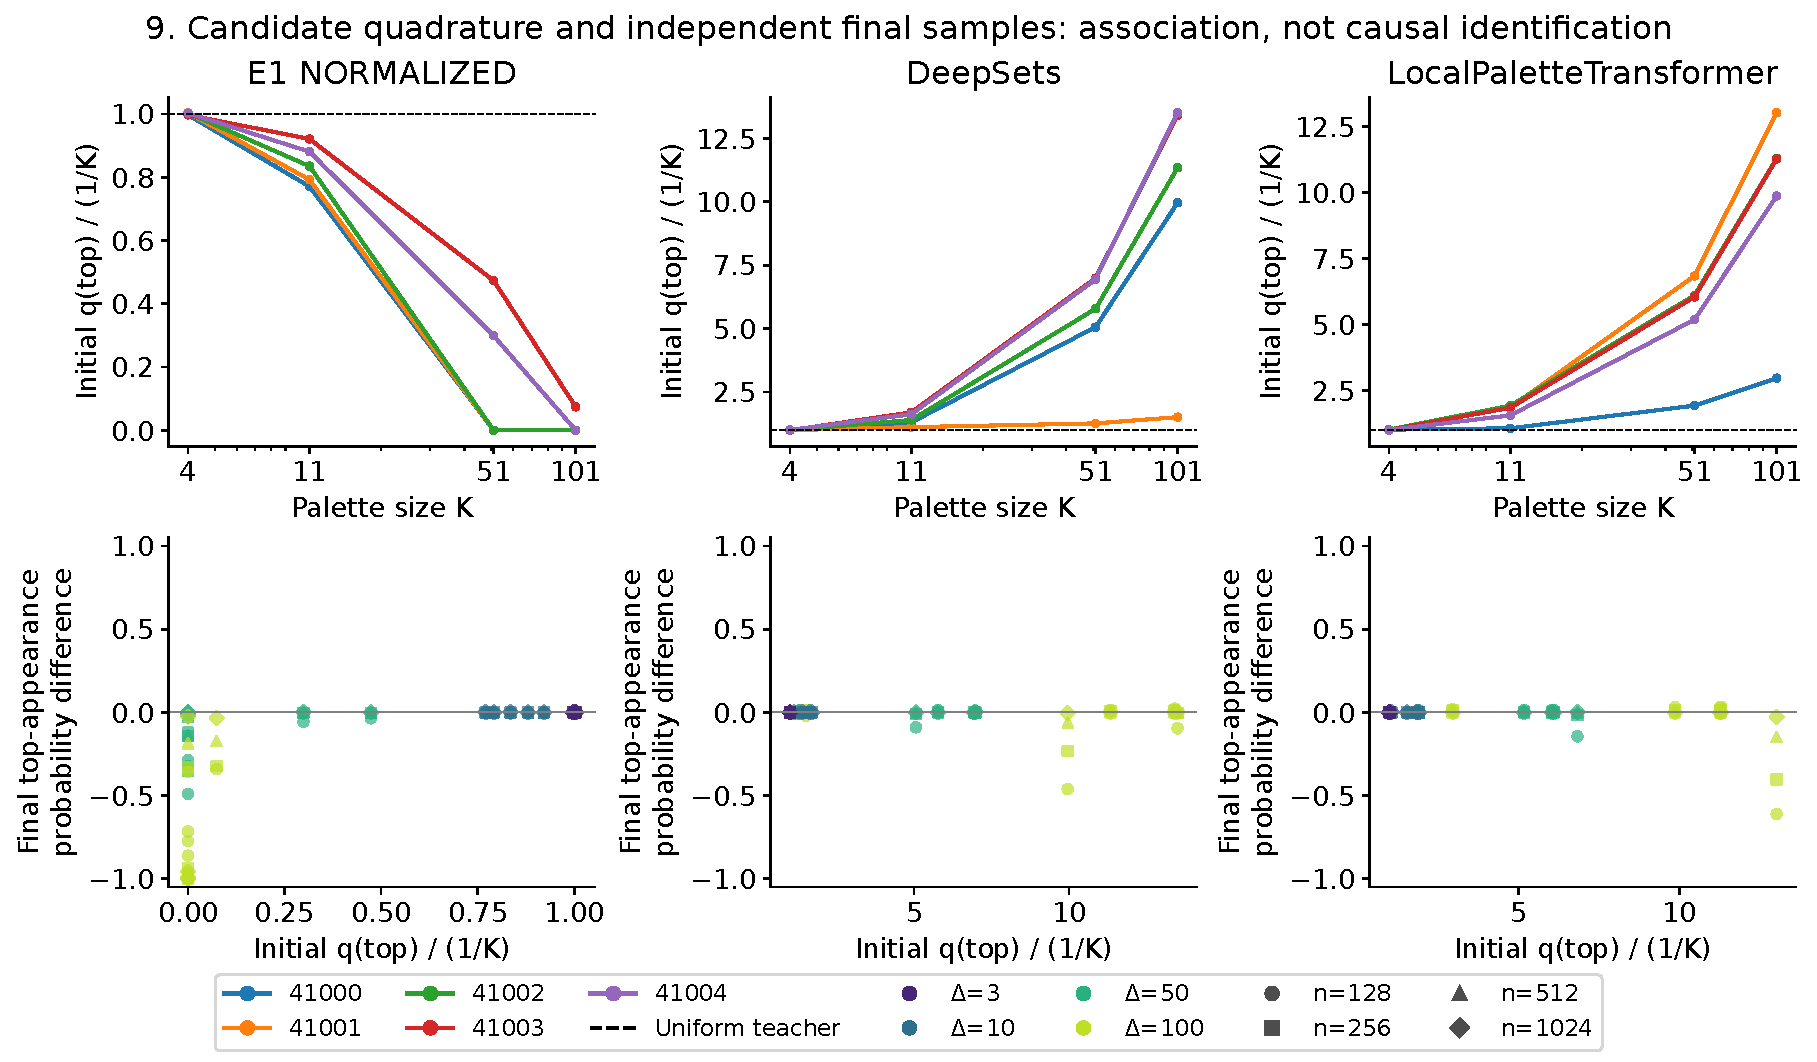
\includegraphics[width=\linewidth,height=.8\textheight,keepaspectratio]{figures/factorial-09-candidates-and-global-law.pdf}
\caption{Same-state candidate quadrature and independent final samples: association does not identify causality.}
\label{fig:factorial-candidates}
\end{figure}

\begin{figure}[p]
\centering
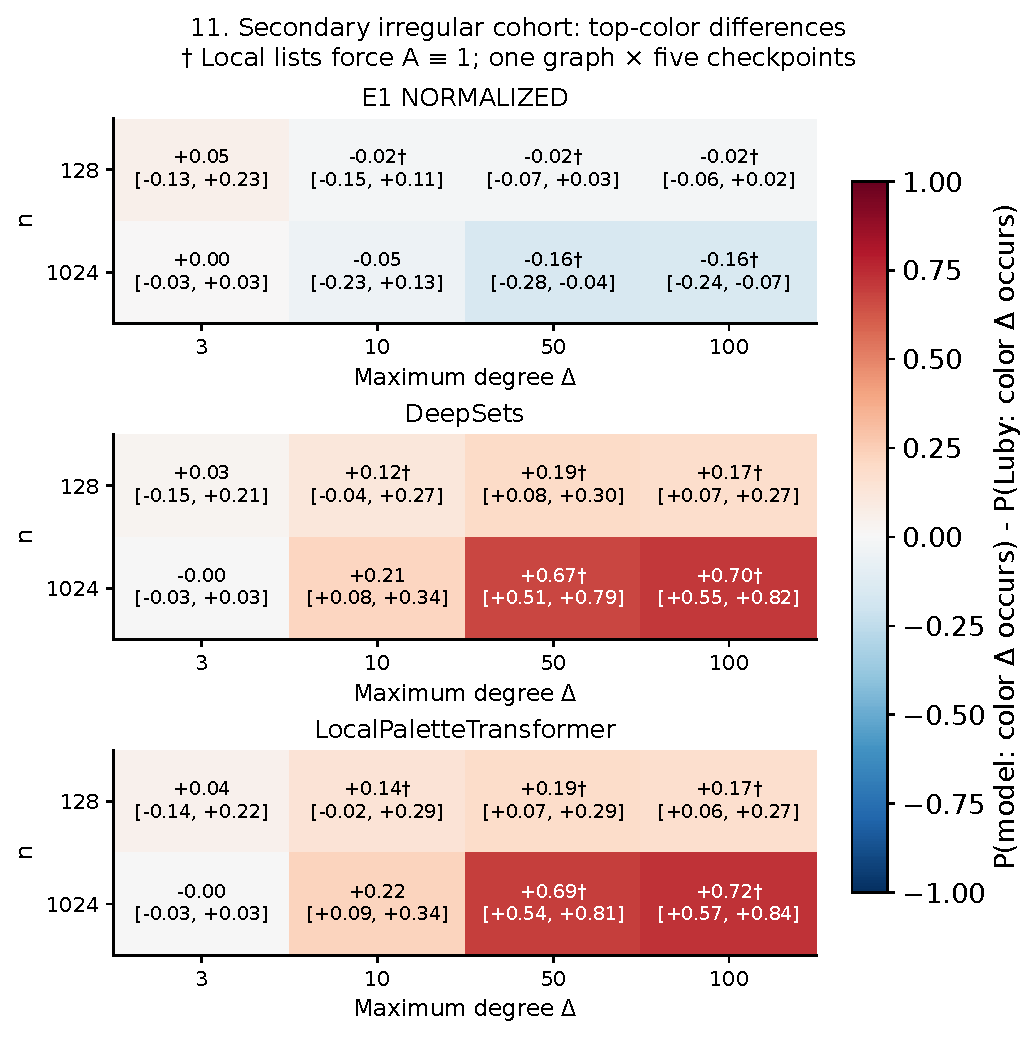
\includegraphics[width=\linewidth,height=.8\textheight,keepaspectratio]{figures/factorial-11-irregular-cohort.pdf}
\caption{Separate irregular cohort: top-color appearance risk differences and simultaneous CP envelopes, averaged over the five fixed checkpoints. A dagger marks list profiles that force the missing-color event A to be true under every completed generator. All eight graphs are retained.}
\label{fig:factorial-irregular}
\end{figure}

\begin{figure}[p]
\centering
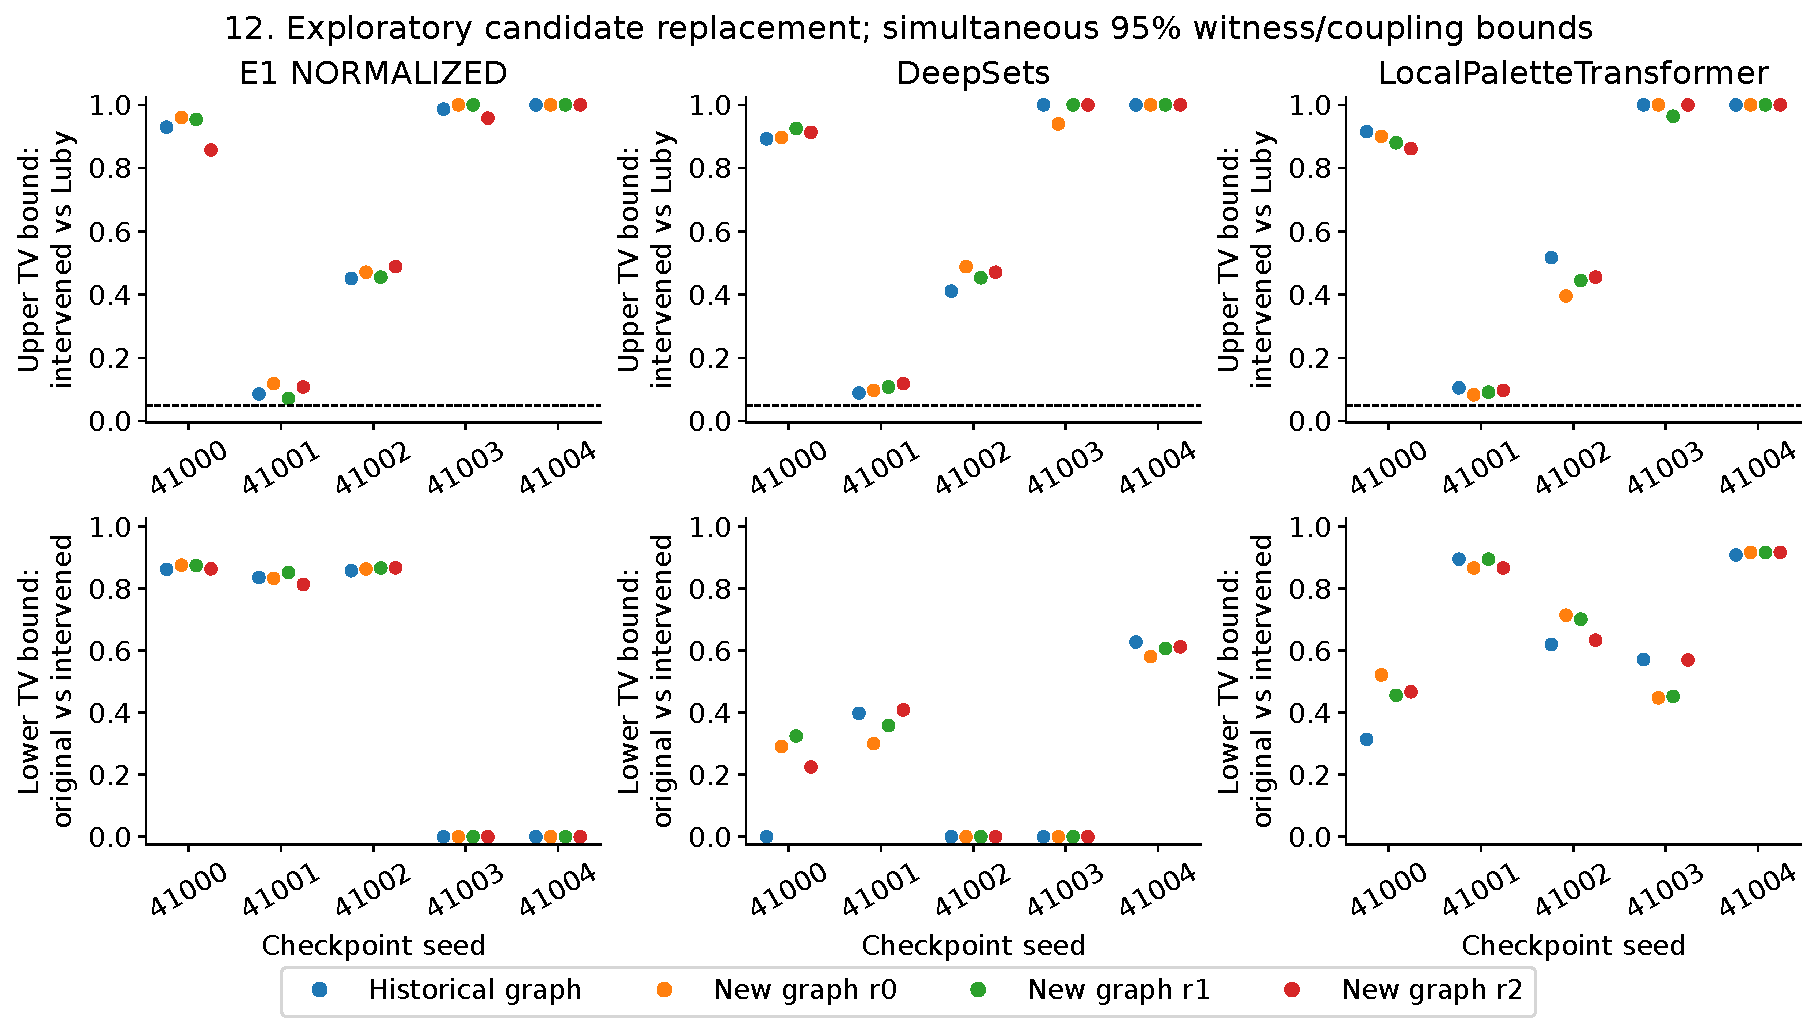
\includegraphics[width=\linewidth,height=.8\textheight,keepaspectratio]{figures/factorial-12-candidate-intervention.pdf}
\caption{Separate exploratory candidate-channel intervention on four priority graphs. The supplementary witness/coupling family gives simultaneous 95 percent upper bounds for intervened versus Luby and lower effect bounds for original versus intervened. All original-policy tests remain separate.}
\label{fig:factorial-intervention}
\end{figure}

\begin{figure}[p]
\centering
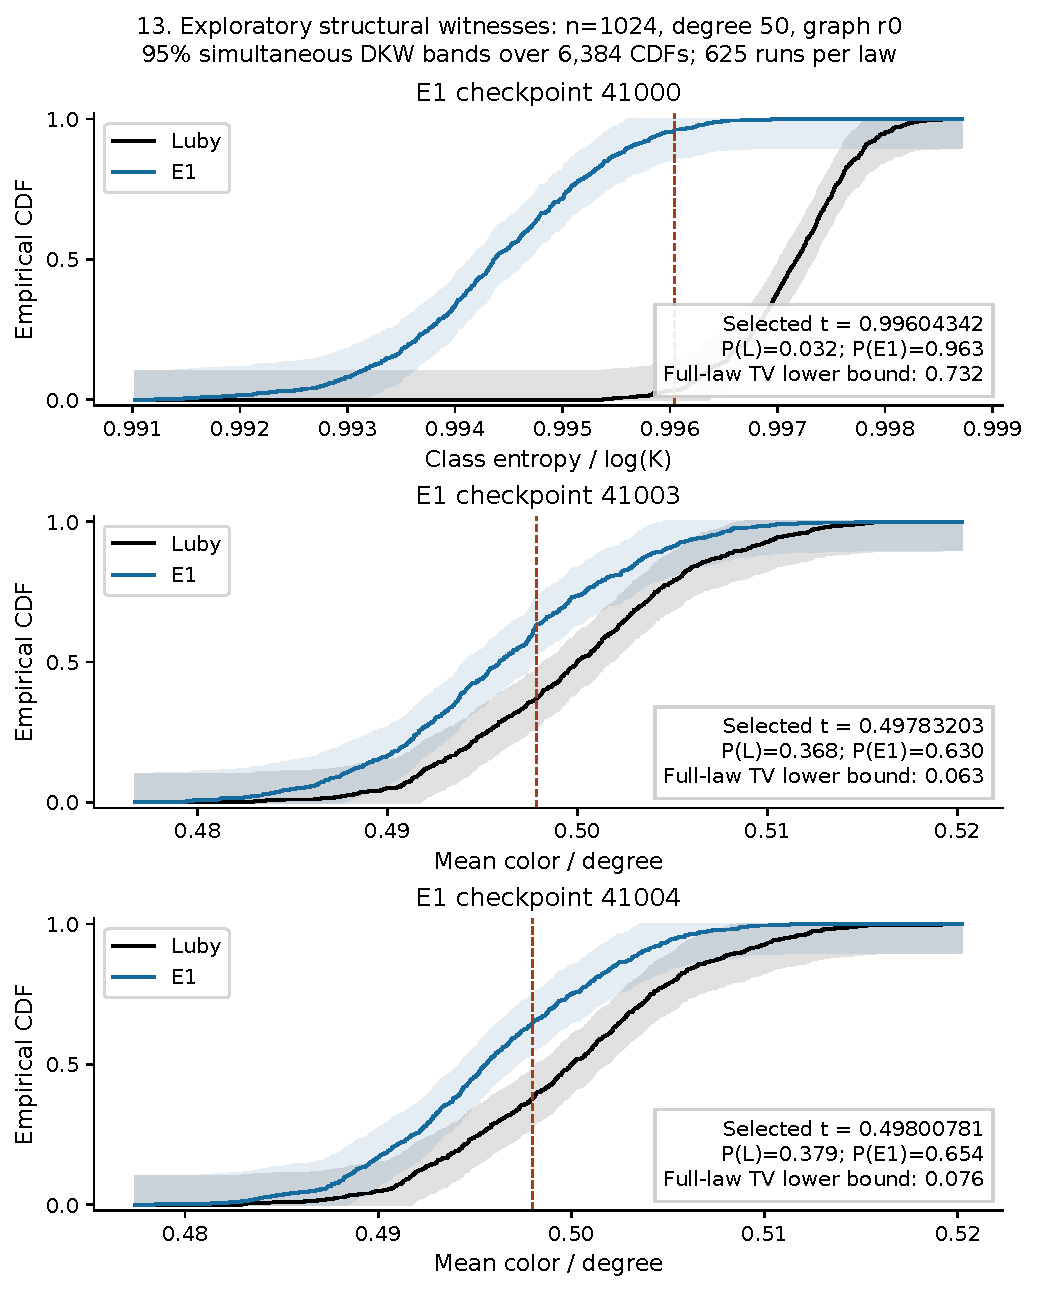
\includegraphics[width=\linewidth,height=.8\textheight,keepaspectratio]{figures/factorial-13-exploratory-cdf-witnesses.pdf}
\caption{Exploratory structural CDF witnesses on one fixed graph, with three E1 checkpoints shown separately. Shaded DKW bands cover all thresholds and all 6,384 predefined graph/generator/function CDFs simultaneously with probability at least .95. Dashed thresholds are selected within this covered family. All 625 original runs per law are used; this is not an independent confirmatory analysis.}
\label{fig:factorial-cdf}
\end{figure}

\clearpage
